\documentclass[10pt, a4paper]{article}
\usepackage{fullpage}
\usepackage{graphicx}
\usepackage{subcaption}

\DeclareGraphicsExtensions{.jpg, .png}

\setlength{\parskip}{0.3cm}
\setlength{\parindent}{0cm}

\begin{document}
\title{Quality Assurance
\\ 3D Heap Visualisation}
\author{Briony Goldsack, Aviv Beeri, Ying Jiang, Oliver Myerscough, 
\\ Anna Thomas, Eleanor Vincent}
\maketitle

\section{Introduction} 
An object-oriented software application creates complex structures on the heap during its lifetime. Debugging object-oriented software often involves thinking about how the heap evolves as a program runs. The aim of our group project is to design a tool which supports visualisation of the heap of a running Java program as a 3D scene which can be navigated by the software developer by moving around as if in a first person shooter game. 

In this report we discuss how we are assuring the quality of our end product.

\section{Version Control}

Git is the obvious choice for our version control needs. The whole group are familiar with git, so using it is pure benefit. Our project is hosted on github. 

\section{Testing}

We are using JUnit and TTD as we build our system.

Our build system, gradle, can be integrated easily with JUnit by using the java plugin. All our tests can be run using the "test" task. The "build" task, which compiles all our code and packages it into a jar depends upon the "test" task. As a result, gradle will not build the project if there are failing tests unless the "tests" task is manually excluded.

After running tests, gradle produces html formatted reports which make it very easy to get both a general overview of the test results and look at particular tests.

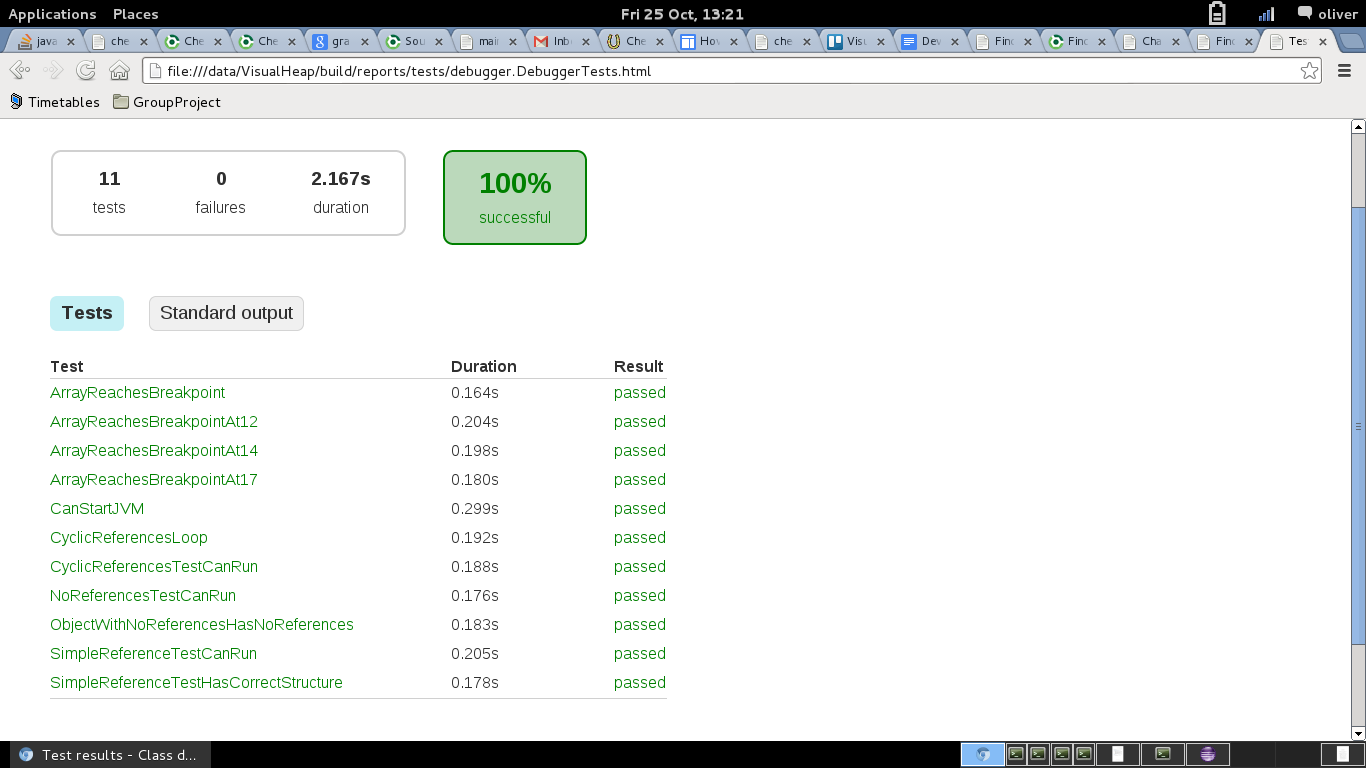
\includegraphics[width=\textwidth]{images/testresults}

\begin{thebibliography}{9}


\end{thebibliography}

\end{document}
